% !TeX spellcheck = en_US
\documentclass[conference]{IEEEtran}
\IEEEoverridecommandlockouts
% The preceding line is only needed to identify funding in the first footnote. If that is unneeded, please comment it out.
\usepackage{cite}
\usepackage{amsmath,amssymb,amsfonts}
%\usepackage{algorithmic}
\usepackage{graphicx}
\usepackage{array}


\usepackage{subcaption}
\renewcommand{\thesubfigure}{\alph{subfigure}}
\captionsetup[subfigure]{labelformat=parens,labelsep=space}

\usepackage{epstopdf}
\usepackage{textcomp}
\usepackage{verbatim}
\usepackage[table]{xcolor}
\usepackage{url}
\usepackage{algorithm}
\usepackage{multirow}
\usepackage{cancel}
\usepackage{xargs}   
\usepackage{colortbl}
\usepackage{amsthm}
\usepackage{pifont}
\usepackage{booktabs,tabularx,makecell}
\usepackage{enumitem}

\usepackage{tikz}
\usetikzlibrary{fit,backgrounds}  
\usetikzlibrary{positioning,arrows.meta}

\renewcommand{\arraystretch}{1.3}
\renewcommand\cellalign{lc}   % makecell default: left-aligned, centred vertically

% Use more than one optional parameter in a new commands

% --- Agent Card listing style ---
\usepackage{listings}
\usepackage{xcolor}
\definecolor{cardbg}{RGB}{249,249,250}
\definecolor{cardstr}{RGB}{166,72,40}   % strings (coral)
\definecolor{cardlit}{RGB}{45,90,150}   % literals (blue)
\definecolor{cardrule}{RGB}{205,205,205}
\lstdefinelanguage{ojson}{
  morestring=[b]{"}, stringstyle=\color{cardstr},
  morekeywords={true,false,null}, keywordstyle=\color{cardlit},
  sensitive=true}
\lstdefinestyle{agentcard}{
  language=ojson, basicstyle=\ttfamily\scriptsize,
  backgroundcolor=\color{cardbg},
  frame=single, rulecolor=\color{cardrule}, framesep=4pt,
  numbers=left, numberstyle=\tiny\color{gray}, numbersep=5pt,
  breaklines=true, breakatwhitespace=true,
  postbreak=\mbox{\textcolor{gray}{$\hookrightarrow$}\,},
  showstringspaces=false, columns=fullflexible, keepspaces=true, tabsize=2}

% --- ReAct trace role colors ---
\definecolor{roleplan}{RGB}{24,95,165}    % blue  - plan/retrieve/validate
\definecolor{rolethink}{RGB}{83,74,183}   % purple- thought
\definecolor{roleact}{RGB}{186,117,23}    % amber - action
\definecolor{roleobs}{RGB}{59,109,17}     % green - observe/deploy
\definecolor{roleneutral}{RGB}{110,110,105} % gray - intent/result

% --- Layered ReAct trace box ---
\usepackage[most]{tcolorbox}
\tcbuselibrary{skins,breakable}
\newtcolorbox{awstep}[2]{%
  enhanced, breakable, sharp corners, boxrule=0pt,
  left=50pt, right=4pt, top=2pt, bottom=2pt,
  colback=#2!7, colframe=#2!7,
  borderline west={2pt}{0pt}{#2},
  fontupper=\ttfamily\scriptsize,
  overlay={\node[anchor=west, text=#2,
                 font=\sffamily\bfseries\fontsize{7.5}{8}\selectfont]
           at ([xshift=5pt]frame.west) {#1};},
  before skip=0pt, after skip=0pt, boxsep=0pt,
}

\usepackage{algpseudocode}
\algnewcommand\algorithmicforeach{\textbf{for each}}
\algdef{S}[FOR]{ForEach}[1]{\algorithmicforeach\ #1\ \algorithmicdo}
\usepackage{setspace}

%\usepackage[colorinlistoftodos,prependcaption,textsize=small]{todonotes}
%\newcommandx{\Dang}[2][1=]{\todo[inline,linecolor=blue,backgroundcolor=blue!25,bordercolor=blue,#1]{Dang: #2}}
%\newcommandx{\Riku}[2][1=]{\todo[inline,linecolor=red,backgroundcolor=red!25,bordercolor=red,#1]{Riku: #2}}
%\newcommandx{\Shahida}[2][1=]{\todo[inline,linecolor=orange,backgroundcolor=orange!25,bordercolor=red,#1]{TaoChen: #2}}

\usepackage{comment}
% *** GRAPHICS RELATED PACKAGES ***
%
\ifCLASSINFOpdf
\else
\fi

\setlength {\marginparwidth }{2cm} 

\begin{document}

\title{\emph{AppWeaver}: Agentic Discovery and Composition of O-RAN Apps for AI-Native 6G}

\author{Yongchao~Dang,
        Tao Chen, 
        and  Riku Jäntti
\thanks{
Yongchao Dang and Riku Jäntti are with the Department of Information and Communications Engineering, School of Electrical Engineering, Aalto University, 02150 Espoo, Finland (e-mail: firstname.lastname@aalto.fi).

Tao Chen is with VTT Technical Research Centre of Finland, 02150 Espoo, Finland (e-mail: tao.chen@vtt.fi).
}
}

\maketitle



\begin{abstract}
Open RAN (O-RAN) opens the radio access network to a growing ecosystem of third-party rApps and xApps, allowing radio resource optimization through standardized Non-Real-Time (Non-RT) and Near-Real-Time (Near-RT) RAN Intelligent Controllers (RICs). However, building O-RAN services for emerging 6G verticals, such as connected vehicles and immersive VR/XR, remains difficult because operators must still manually discover suitable applications, understand their dependencies, configure and validate them, and coordinate them into end-to-end workflows. This article introduces \emph{AppWeaver}, an agentic-AI framework that orchestrates end-to-end O-RAN workflows by using LLM-based agents to interpret operator intent, query an Agent Card registry that describes each xApp and rApp in terms of its functions, properties, and interfaces, reason about their capabilities and dependencies, and compose them into ordered, service-specific workflows. In addition, \emph{AppWeaver} confines LLM agents to workflow-level orchestration over existing xApps and rApps, rather than direct RAN control, preserving a clear control-plane boundary in which native RIC applications execute low-level RAN control and monitoring actions, while agent-generated workflows are evaluated against operator policies, security constraints, validation outcomes, and rollback requirements. The resulting workflows are orchestrated with LangGraph, coordinated via Agent-to-Agent (A2A) communication, connected to xApps and rApps through Model Context Protocol (MCP) tool bindings, and validated in a FlexRIC and OpenAirInterface test environment.
\end{abstract}

\begin{IEEEkeywords}
O-RAN, agentic AI, large language models (LLMs), workflow composition.
\end{IEEEkeywords}

\IEEEpeerreviewmaketitle

\section{Introduction}\label{sec:sec1} 
Upcoming 6G networks will evolve into programmable, artificial intelligence (AI)-native platforms for immersive, sensing, and edge-intelligence services, whose diverse requirements demand flexible and service-aware RAN automation~\cite{polese2026beyond}. To provide this flexibility, the O-RAN ALLIANCE\footnote{\url{https://www.o-ran.org/}} defines a disaggregated and programmable RAN architecture with standardized open interfaces and hierarchical RAN Intelligent Controllers (RICs), where rApps in the Non-Real-Time (Non-RT) RIC support long-term optimization and policy guidance, while xApps in the Near-Real-Time (Near-RT) RIC provide near-real-time RAN control~\cite{almeida2023ric}.
This openness reduces vendor lock-in and enables an open ecosystem of interoperable third-party xApps and rApps for service-specific RAN automation, providing end users with more adaptive, service-aware connectivity.


Building on this openness, Hexa-X-II\footnote{\url{https://hexa-x-ii.eu/}} advances intent-based management for 6G operations, where operator intents are realized through the available xApps and rApps. However, as the application catalog grows, realizing intents across a multi-vendor ecosystem raises three open problems. First, an intent must be mapped to the right xApps, rApps, APIs, and control procedures, but O-RAN defines application exposure rather than intent-driven selection and composition\footnote{\url{https://www.o-ran.org/specifications}}, leaving this step manual. Second, an intent may span multiple applications that depend on shared data, models, policies, and control actions, yet these dependencies are still validated in separate steps across design, deployment, and runtime. Third, an intent can trigger automated control, but conflict mitigation, authorization, lifecycle control, auditing, rollback, and human approval are not tied together into one governed execution path. These gaps make intent realization difficult to scale and govern in open, multi-vendor O-RAN systems.

\begin{table*}[t]
\centering
\caption{Classification of representative agentic O-RAN systems by capability.}
\label{tab:positioning}
\footnotesize
\setlength{\tabcolsep}{5pt}
\begin{tabular}{@{}llccccccl@{}}
\toprule
\multirow{2}{*}{\textbf{System}} & \multirow{2}{*}{\textbf{Control paradigm}} & \multirow{2}{*}{\textbf{Intent}} & \multicolumn{2}{c}{\textbf{Reuse \& composition}} & \multicolumn{3}{c}{\textbf{Conflict \& assurance}} & \multirow{2}{*}{\textbf{Evaluation}} \\
\cmidrule(lr){4-5}\cmidrule(lr){6-8}
 & & & \textbf{Disc.} & \textbf{Comp.} & \textbf{Confl.} & \textbf{Valid.} & \textbf{Adapt.} & \\
\midrule
RIC-O~\cite{almeida2023ric}       & Optimization-based RIC placement   & \ding{55} & \ding{55} & \ding{55} & \ding{55} & \ding{55} & $\sim$ & Kubernetes \\
AutoRAN~\cite{maxenti2026autoran} & LLM-driven deployment automation   & \ding{51} & \ding{55} & $\sim$ & \ding{55} & \ding{51} & $\sim$ & OAI/srsRAN/ARC \\
OREO~\cite{mungari2025ran}        & Optimization-based xApp deployment & \ding{55} & $\sim$ & $\sim$ & $\sim$ & \ding{55} & \ding{55} & Colosseum emulator \\
RAN assurance~\cite{singh2025agentic} & Multi-agent assurance          & $\sim$ & \ding{55} & $\sim$ & \ding{51} & \ding{51} & \ding{51} & Simulation \\
AGORAN~\cite{chatzistefanidis2025agoran} & Multi-agent intent negotiation & \ding{51} & $\sim$ & \ding{55} & \ding{51} & \ding{55} & $\sim$ & OAI/FlexRIC \\
AgentRAN~\cite{elkael2026agentran} & Hierarchical multi-agent control  & \ding{51} & \ding{55} & $\sim$ & $\sim$ & $\sim$ & \ding{51} & OAI (OTA) \\
Multi-scale~\cite{navidan2026toward} & Multi-timescale multi-agent control & \ding{51} & \ding{55} & \ding{55} & $\sim$ & \ding{55} & \ding{51} & Architecture \\
Multi-agentic rApp~\cite{li2026multi} & Multi-agent policy control     & \ding{51} & \ding{55} & $\sim$ & \ding{51} & $\sim$ & $\sim$ & Simulation \\
MX-AI~\cite{chatzistefanidis2025mxai} & Multi-agent observability and control & \ding{51} & \ding{55} & $\sim$ & \ding{55} & $\sim$ & $\sim$ & OAI/FlexRIC \\
\midrule
\rowcolor{gray!12}
\textbf{AppWeaver (ours)} & \textbf{Multi-agent workflow orchestration} & \ding{51} & \ding{51} & \ding{51} & \ding{51} & \ding{51} & $\sim$ & OAI/FlexRIC \\
\bottomrule
\end{tabular}
\begin{minipage}{\textwidth}
\vspace{2pt}
\footnotesize
\emph{Control paradigm}: control approach adopted. \emph{Intent}: natural-language interface. \emph{Disc.}: discovery of reusable xApps/rApps. \emph{Comp.}: composition into executable workflows. \emph{Confl.}: cross-application conflict handling. \emph{Valid.}: pre-deployment sandbox or twin validation. \emph{Adapt.}: runtime adaptation and rollback. Marks: \ding{51}~demonstrated or core focus; $\sim$~partial or by-design; \ding{55}~not addressed.
\end{minipage}
\end{table*}



To this end, this paper proposes \emph{AppWeaver}, an agentic-AI framework that orchestrates end-to-end O-RAN workflows by using LLM-based agents to interpret operator intent, discover reusable xApps and rApps, reason about their capabilities and dependencies, and compose them into ordered, service-specific workflows. The main design elements and contributions of \emph{AppWeaver} are summarized as follows.
\begin{itemize}
    \item \textbf{\textit{Agent Card for xApp/rApp.}}     Each xApp and rApp is wrapped by a machine-readable Agent Card\footnote{\url{https://www.agentcard.net/}} that describes its functions, interfaces, control scope, resource demand, dependencies, policy constraints, and MCP tool endpoints. This allows agents to discover, compare, and reuse third-party applications without modifying their internals, while providing the semantic grounding needed for dependency reasoning and compatibility checking. 
    \item \textbf{\textit{Agentic workflow composition.}}   Based on the Agent Card abstraction and the Agentic Resource Discovery (ARD) principle\footnote{\url{https://agenticresourcediscovery.org/}}, LLM agents translate operator intent into workflows by discovering suitable xApps and rApps, reasoning about their capabilities and dependencies, and coordinating execution through A2A communication and a LangGraph-based state machine. This enables reusable O-RAN applications to be selected, connected, and orchestrated for different service requirements without manual workflow construction.
    \item \textbf{\textit{Agentic workflow testing and deployment.}}  Each generated workflow is tested before deployment through interface compatibility checking, policy verification, rollback planning, and human-in-the-loop approval when required. Only validated and approved workflows are deployed through standardized O-RAN interfaces, while operator policies, auditing, and rollback mechanisms keep execution observable, controlled, and reversible.
\end{itemize}

These agentic capabilities enable an intent-to-deployment pipeline that covers application discovery, workflow composition, predeployment validation, and governed execution across reusable O-RAN applications.
The remainder of this paper is organized as follows. Section~\ref{sec:background} reviews related work on agentic AI for O-RAN. Section~\ref{sec:architecture} introduces the AppWeaver architecture. Section~\ref{sec:evaluation} presents the prototype implementation and evaluation with OAI and FlexRIC. Section~\ref{sec:conclusion} concludes the paper and outlines future directions.

\section{Agentic AI for O-RAN}\label{sec:background}
Agentic AI for O-RAN refers to governed LLM-based agents that interpret operator intent, retrieve external knowledge, reason over network context, plan actions, and invoke O-RAN APIs and tools for automation. Unlike traditional rule-based network agents that follow predefined policies and fixed control logic, these agents interpret natural-language instructions and adapt their behavior to dynamic network conditions. Recent work explores this direction from three complementary perspectives, namely xApp and rApp development, O-RAN component deployment and lifecycle management, and intent-driven network automation, summarized in Table~\ref{tab:positioning}.


\subsection{Agentic AI for xApp and rApp Development}
Developing xApps and rApps requires a heavy engineering burden, as each application requires RAN control logic, E2 and A1 service model integration, RIC SDK interfacing, and validation on the target platform. Agentic AI is being leveraged to reduce this burden, with LLM-based agents translating natural-language requirements into application code, service model bindings, configuration artifacts, and test templates, and supporting adaptive reasoning inside xApps for radio resource management~\cite{maatouk2024large}. However, these efforts mainly target the development of individual applications and treat the LLM as a code-generation or reasoning engine, while agentic capabilities such as tool invocation, knowledge retrieval, multi-step planning, and multi-agent collaboration remain underexplored.


\subsection{Agentic AI for O-RAN Deployment and Management}
O-RAN deployment and management involve placing disaggregated functions across cloud-native infrastructure, allocating resources, resolving inter-application conflicts, and verifying behavior before execution. To automate these tasks, existing studies combine optimization, learning-based prediction, and agentic decision-making. RIC-O optimizes the placement of distributed near-RT RIC instances across the cloud-edge continuum through dynamic clustering of radio nodes~\cite{almeida2023ric}, while graph neural network based methods predict conflicts among xApps before deployment~\cite{al2026ran}. AutoRAN translates high-level operator intent into deployment, configuration, and testing artifacts for multi-vendor O-RAN systems~\cite{maxenti2026autoran}, whereas OREO formulates xApp deployment as a joint optimization problem over application selection, function sharing, configuration, and resource allocation~\cite{mungari2025ran}. Assurance-oriented frameworks add explicit verification stages to validate AI-generated decisions before execution~\cite{singh2025agentic}. Although these efforts reduce the operational complexity of deploying and managing O-RAN components, they mainly assume that the candidate applications are already known and focus on their placement, configuration, or validation, rather than on discovering reusable xApps and rApps and assembling them into service-specific workflows.


\subsection{Agentic AI for Intent-Based RAN Automation}
Intent-based RAN automation enables operators to specify high-level service objectives in natural language, which collaborating agents translate into control actions; a key challenge is how such intents are interpreted and resolved in multi-stakeholder settings. AGORAN addresses this challenge through intent negotiation, where LLM-based broker agents reconcile conflicting requirements under governance constraints and translate the agreed outcomes into enforceable policies through standard O-RAN interfaces~\cite{chatzistefanidis2025agoran}.
Building on this direction, subsequent work aligns agent structures and computational models with O-RAN's hierarchical, multi-timescale control loops, as in AgentRAN, which coordinates rApp, xApp, and dApp agents through A2A communication and MCP-based tool invocation~\cite{elkael2026agentran}, and multi-scale frameworks that map LLMs, small language models (SLMs), and wireless foundation models to the Non-RT, Near-RT, and real-time loops to meet heterogeneous latency requirements~\cite{navidan2026toward}. The direction further extends to concrete implementations and system-level demonstrations, including conflict-aware policy generation through collaborative rApp agents~\cite{li2026multi,chatzimiltis2026agentic} and live prototypes such as MX-AI, which provides end-to-end observability and closed-loop control in operational deployments~\cite{chatzistefanidis2025mxai}.

Despite advances in application development, deployment automation, intent understanding, architectural design, and closed-loop execution, existing systems commonly assume that the applications required to realize a service are already known. However, an end-to-end service often requires coordinating multiple reusable applications rather than executing a single xApp or rApp in isolation. For example, traffic steering typically involves KPI monitoring, anomaly detection, QoE prediction, traffic-steering optimization, and RAN control~\cite{yang2024agile}. Current approaches therefore map operator intent to actions over predefined xApps and rApps, but do not address how such applications are discovered in an open, multi-vendor ecosystem, verified for interface and control-scope compatibility, and composed into validated executable workflows. As O-RAN application ecosystems expand and services increasingly span multiple vendors, this gap in application discovery and composition becomes a key barrier to fully autonomous service orchestration, motivating the design of AppWeaver.



\section{AppWeaver Architecture and Workflow}\label{sec:architecture}
\subsection{AppWeaver Architecture} 
Figure~\ref{fig:AppWeaver} shows the AppWeaver architecture, which sits between the operator specifying the intent and the RAN vendors providing the RIC and its xApps and rApps. AppWeaver does not replace existing O-RAN applications but orchestrates them into service-specific workflows through discovery, composition, validation, and governed execution. At its core, a LangGraph-based orchestration layer\footnote{\url{https://www.langchain.com/langgraph}} runs a Planner agent that interprets the operator intent and coordinates four orchestration agents over the A2A bus\footnote{\url{https://a2a-protocol.org/latest/specification/}}. The Discover agent identifies candidate xApps and rApps, the Compose agent assembles them into an ordered workflow, the Validate agent checks the workflow before deployment, and the Deploy agent applies the validated workflow to the RIC. These agents draw on two shared resources, an Agent Registry that stores the Agent Card and endpoint of each available xApp and rApp for capability-based selection, and a shared memory that holds the model state, running summaries, and workflow context across reasoning steps. Within this shared memory, retrieval-augmented generation (RAG) grounds discovery in the registry, a small language model (SLM) supports lightweight reasoning, and a feedback loop lets deployment outcomes refine later decisions.

\begin{figure}[t]
\centering
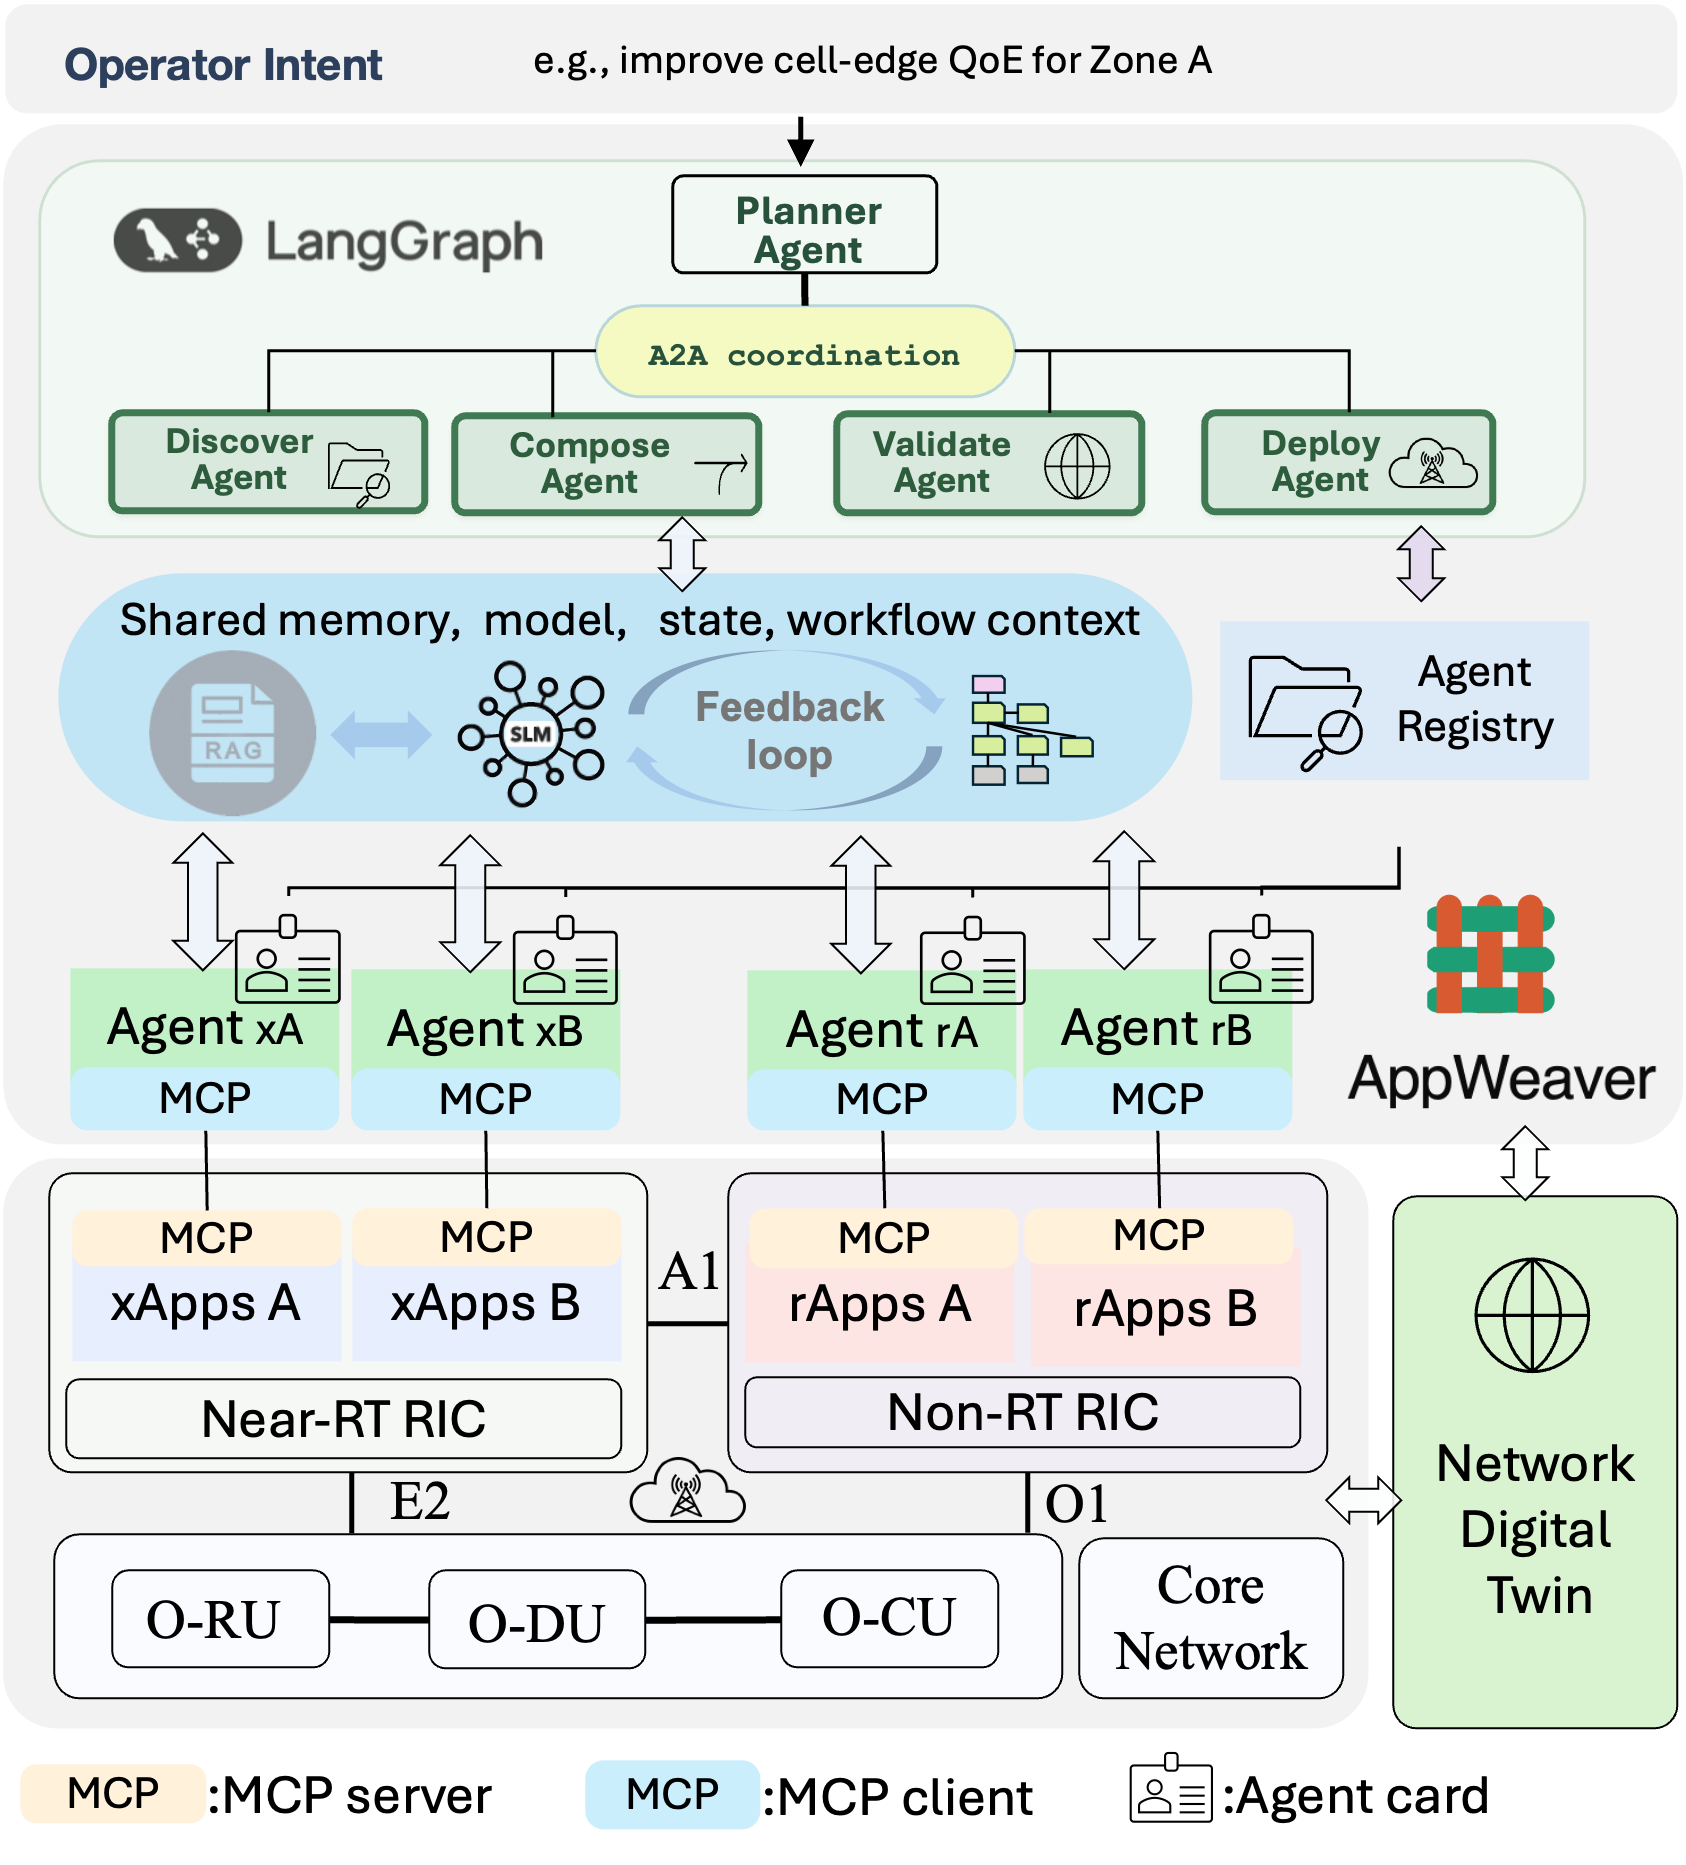
\includegraphics[width=8.0cm]{Pictures/AppWeaver.png}
\caption{AppWeaver architecture.}
\label{fig:AppWeaver}
\end{figure}

AppWeaver operates across two environments, the live RAN and a network digital twin. On the live RAN, a per-application domain agent wraps each selected xApp or rApp and reaches it through an MCP client\footnote{\url{https://modelcontextprotocol.io/specification/}} connected to the MCP server co-located with the application in the Near-RT or Non-RT RIC. The server exposes monitoring and control functions as callable tools, so the domain agent orchestrates the workflow while the application executes the E2 and A1 control actions. In parallel, the Validate agent connects to a network digital twin that mirrors the per-layer RAN state as a live replica. Each candidate workflow is first exercised on the twin to estimate target KPI impact and detect conflicts or errors, so only validated workflows are applied to production. This separation gives AppWeaver a safety boundary by testing workflows before they reach the live RAN, while keeping all E2 and A1 control actions within existing xApps and rApps and their native control loops.


\subsection{AppWeaver Workflow}
The AppWeaver workflow follows a reasoning-and-acting (ReAct) loop, illustrated in Fig.~\ref{fig:trace} for a cell-edge QoE intent, and moves through four stages, discovery, composition, validation, and deployment, all driven by the LLM-based agents in the AppWeaver core. Given an operator intent, the Planner agent interprets the request, extracts the target objective, constraints, and affected zone, and decomposes the intent into subgoals. The Discover agent then retrieves candidate applications from the Agent Registry, matching subgoals to advertised capabilities rather than names. For the cell-edge QoE objective (skill \texttt{analyze\_qoe}), it selects a KPM-monitoring xApp for live radio KPIs, a QoE-prediction rApp for estimating user experience, a mobility-optimization rApp for adjusting handover behavior, and a QoS-control xApp for scheduling and priority changes.

\begin{figure}[htbp]
\centering
\begin{awstep}{intent}{roleneutral}Improve cell-edge QoE for Zone A; skill = analyze\_qoe.\end{awstep}
\begin{awstep}{discover}{roleplan}RAG over Agent Registry $\rightarrow$ kpm-mon.xApp, qoe-pred.rApp, mobility-opt.rApp, qos-ctrl.xApp.\end{awstep}
\begin{awstep}{thought}{rolethink}Edge QoE unknown; read live KPIs first.\end{awstep}
\begin{awstep}{action}{roleact}get\_kpi \{ zone: "A" \}\end{awstep}
\begin{awstep}{observe}{roleobs}\{ prb\_util: 0.87, sinr\_edge\_db: 3.1, edge\_ues: 14 \}\end{awstep}
\vspace{1.5pt}
\begin{awstep}{thought}{rolethink}Load high, edge SINR low; forecast QoE, find at-risk UEs.\end{awstep}
\begin{awstep}{action}{roleact}predict\_qoe \{ zone: "A" \}\end{awstep}
\begin{awstep}{observe}{roleobs}\{ qoe\_mos: 2.8, at\_risk\_ues: 11, bottleneck: "edge\_sinr" \}\end{awstep}
\vspace{1.5pt}
\begin{awstep}{thought}{rolethink}Relieve edge: rebalance mobility, then raise priority.\end{awstep}
\begin{awstep}{action}{roleact}optimize\_handover \{ zone: "A" \}; set\_priority \{ class: "edge", weight: "high" \}\end{awstep}
\begin{awstep}{observe}{roleobs}\{ policy: "ho\_margin +3 dB; steer 4 UEs $\rightarrow$ CS-7" \}\end{awstep}
\vspace{1.5pt}
\begin{awstep}{validate}{roleplan}Twin what-if $\rightarrow$ \{ pred\_qoe\_mos: 3.6, conflicts: 0 \}: pass.\end{awstep}
\begin{awstep}{deploy}{roleobs}Commit the validated policy over E2SM-RC to the live RAN; monitoring on.\end{awstep}
\begin{awstep}{result}{roleneutral}Cell-edge QoE MOS 2.8 $\rightarrow$ 3.6; validated workflow deployed.\end{awstep}
\caption{AppWeaver ReAct trace for the cell-edge QoE intent.}
\label{fig:trace}
\end{figure}



The Compose agent turns these applications, their tool schemas, and the operator constraints into an ordered workflow, which then executes under the same ReAct loop. As the trace in Fig.~\ref{fig:trace} shows, the loop first reads live KPIs for Zone A through the monitoring xApp, namely PRB utilization, edge SINR, and the edge UE count. It uses these observations to invoke the QoE-prediction rApp, estimating MOS and identifying at-risk UEs before any control decision. Guided by the prediction, it selects corrective actions, mobility rebalancing and higher scheduling priority for edge users, and maps them to the tools exposed by the mobility-optimization rApp and the QoS-control xApp. Each action, whether an A2A message between agents or an MCP tool call to an application, returns an observation that is written back into the shared state, so the workflow adapts step by step to the latest KPIs, predictions, and outcomes rather than running as a fixed pipeline. Finally, the Validate agent evaluates the candidate workflow on the digital twin and interprets its expected KPI impact and any conflicts, and once validation succeeds, the Deploy agent commits it to the live RAN with monitoring kept active.

% NOTE: the next two lines belong in the preamble after \usepackage{subcaption}.
% They are kept here only if this section is compiled standalone.
%\renewcommand{\thesubfigure}{\alph{subfigure}}
%\captionsetup[subfigure]{labelformat=parens,labelsep=space}

\begin{figure*}[t]
  \centering
  \begin{subfigure}[b]{0.25\textwidth}
    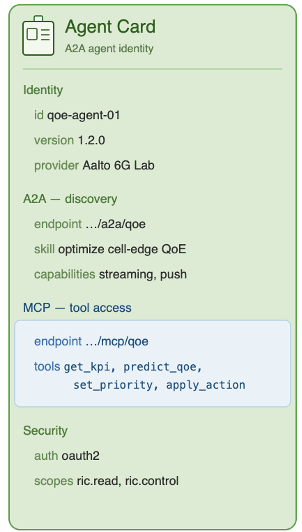
\includegraphics[width=\linewidth]{Pictures/Agent_card.png}
    \caption{Agent Card}
    \label{fig:agentcard}
  \end{subfigure}\hfill
  % Revision (R4 minor, Fig. 3 density): the MCP-server panel (Pictures/MCP.png) is removed; its
  % tools/list and tools/call exchange is shown in the discovery sequence, now printed larger.
  \begin{subfigure}[b]{0.72\textwidth}
    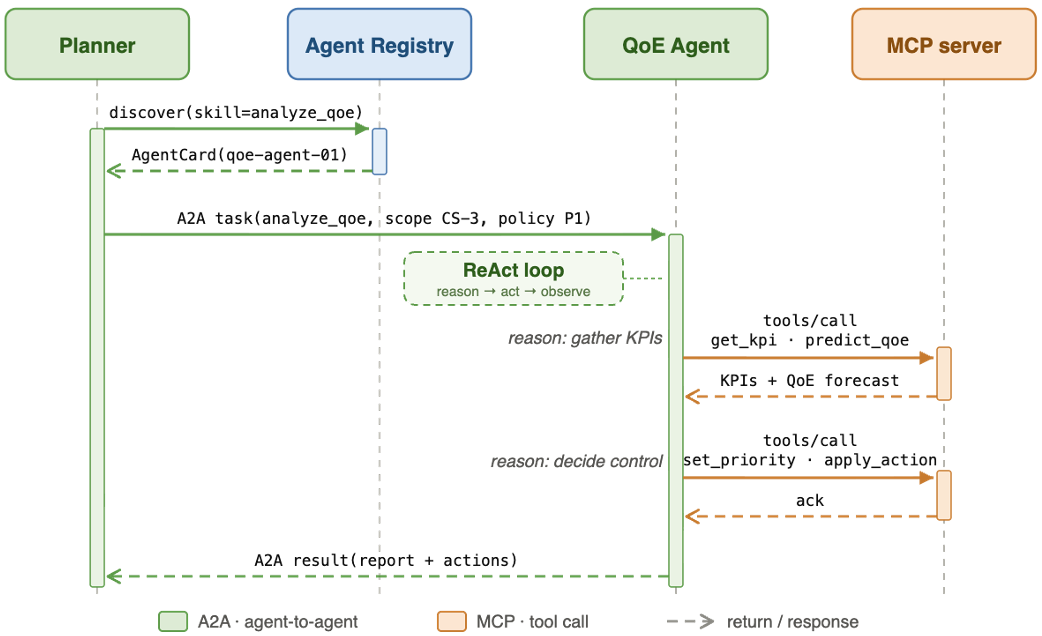
\includegraphics[width=\linewidth]{Pictures/UML.png}
    \caption{Discovery and invocation sequence (A2A and MCP)}
    \label{fig:sequence}
  \end{subfigure}
  \caption{AppWeaver agent interfaces and procedure.}
  \label{fig:appweaver-agent}
\end{figure*}

\subsection{Agent Interfaces and Procedure}
Figure~\ref{fig:appweaver-agent} details the AppWeaver interfaces for exposing, discovering, and invoking third-party xApps and rApps, using the cell-edge QoE intent as an example. Fig.~\ref{fig:appweaver-agent}(a) shows the Agent Card, a machine-readable JSON descriptor registered in the Agent Registry that lets AppWeaver treat each xApp or rApp as a discoverable and reusable component. It specifies the application's capabilities, such as KPI monitoring, QoE prediction, mobility optimization, or QoS control; supported interfaces and data models, including E2SM-KPM, E2SM-RC, and A1 policy types; control scope over cells, slices, UEs, and tunable parameters; and resource requirements, operational constraints, and MCP tool endpoints used to monitor, configure, and control the RAN through the underlying application. Because this description is maintained outside the application, AppWeaver translates operator intent into RAN control through existing xApps and rApps without modifying their internal logic or driving O-RAN interfaces directly. A new application is onboarded by registering its Agent Card.

The MCP steps of Fig.~\ref{fig:appweaver-agent}(b) show how a domain agent invokes application tools through an MCP client connected to the MCP server co-located with its xApp or rApp. The agent first sends a \texttt{tools/list} request to discover available monitoring and control tools, then issues \texttt{tools/call} requests to invoke selected tools, such as \texttt{get\_kpi} and \texttt{predict\_qoe} for observation, and \texttt{set\_priority} and \texttt{apply\_action} for control. The MCP server translates these calls to the underlying application, and the xApp or rApp executes RAN operation over E2 or A1. This keeps the agent at the orchestration level, hides vendor-specific management APIs behind a uniform tool interface, and makes each external operation, whether telemetry collection, invocation, or policy update, an explicit typed action that can be logged, validated, and replayed.

Using Agent Cards and MCP tools, the orchestration agents search the Agent Registry, select suitable domain agents, and assign tasks over the A2A coordination plane, as shown by the A2A steps of Fig.~\ref{fig:appweaver-agent}(b). For the cell-edge QoE intent, the Discover agent queries the registry for the required skill and receives matching Agent Cards, including the QoE agent and its endpoints. The Planner agent then assigns the QoE agent an A2A task carrying the objective, scope, and policy constraints. The QoE agent runs the ReAct loop in Fig.~\ref{fig:trace} by calling MCP tools to gather KPIs and a QoE forecast, reasoning over the results, applying selected control actions, and returning an A2A result with the report and actions to the Planner agent. This separation turns a high-level intent into concrete, traceable tool invocations without orchestration agents directly touching O-RAN interfaces.


The Agent Card and MCP abstractions expose heterogeneous xApps and rApps as discoverable, reusable agents, and the ReAct loop composes them through iterative reasoning, tool invocation, and observation into a validated workflow. AppWeaver serves as an intent-translation layer between the operator and vendor-provided RIC applications, mapping high-level objectives onto existing xApps and rApps through their agent interfaces. This layering separates timescales, with AppWeaver orchestrating at seconds to minutes while the applications retain native E2 and A1 control in their own loops, keeping orchestration separate from control execution.


\section{AppWeaver Evaluation}\label{sec:evaluation}
\subsection{Prototype Setup}
Fig.~\ref{fig:testbed} shows the AppWeaver testbed, built on OpenAICellular\footnote{\url{https://www.openaicellular.org/}}. The orchestration host runs the AppWeaver LangGraph orchestrator alongside the FlexRIC Near-RT RIC, and a separate GPU server hosts the gpt-oss planner\footnote{\url{https://huggingface.co/openai/gpt-oss-120b}} via Ollama\footnote{\url{https://github.com/ollama/ollama}}. The RAN includes a live network, with an OAI gNB, a 5G core, and RF-simulated UEs, and a RAN emulator that acts as a digital twin, with FlexRIC connected to both over E2 so the same xApps can run against the live network or the twin. Built on the micro-SDK abstraction of the RAN pipeline~\cite{schmidt2021ran}, the twin mirrors the live RAN through MAC, RLC, and PDCP state synchronization and exposes the same control-plane APIs, so composed workflows can be validated before deployment. Although OpenAICellular provides the base functionality for this testbed, it includes only a small set of xApps and rApps. To expand AppWeaver's application catalog, an agentic coding workflow based on OpenAI Codex\footnote{\url{https://openai.com/codex/}} was used to develop four additional FlexRIC xApps in Python 3.10, covering KPM monitoring, QoE prediction, mobility optimization, and QoS control. rApps typically require a large, live-scale network, so in this testbed they are emulated as test endpoints with standardized APIs rather than deployed as production systems, and are left for future work in collaboration with industry partners.

\begin{figure}[t]
\centering
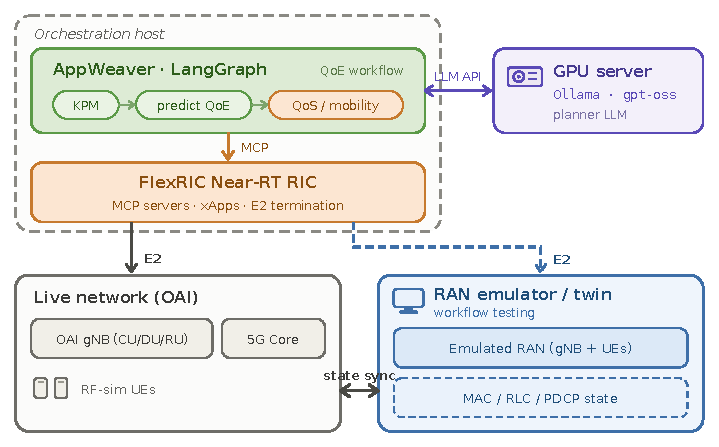
\includegraphics[width=\columnwidth]{Pictures/appweaver_testbed.pdf}
\caption{AppWeaver prototype testbed.}
\label{fig:testbed}
\end{figure}



\begin{figure*}[t]
  \centering
  \begin{subfigure}[b]{0.31\textwidth}
    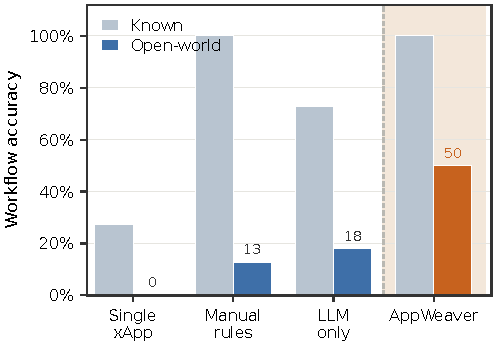
\includegraphics[width=\linewidth]{Pictures/appweaver_accuracy.pdf}
    \caption{Workflow accuracy}
    \label{fig:eval_accuracy}
  \end{subfigure}\hfill
  \begin{subfigure}[b]{0.35\textwidth}
    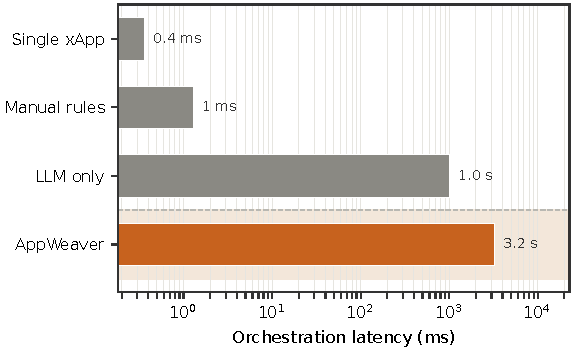
\includegraphics[width=\linewidth]{Pictures/appweaver_latency.pdf}
    \caption{Orchestration latency}
    \label{fig:eval_latency}
  \end{subfigure}\hfill
  \begin{subfigure}[b]{0.31\textwidth}
    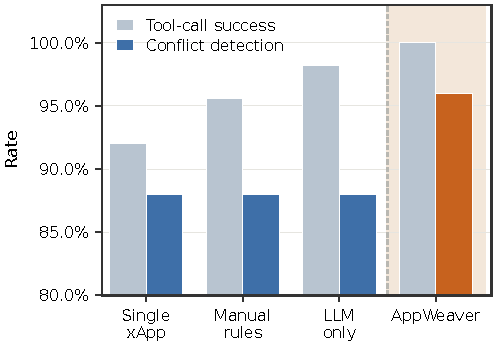
\includegraphics[width=\linewidth]{Pictures/appweaver_reliability.pdf}
    \caption{Reliability}
    \label{fig:eval_reliability}
  \end{subfigure}
  \caption{AppWeaver versus baselines on workflow accuracy, orchestration latency, and reliability.}
  \label{fig:appweaver_eval}
\end{figure*}


\subsection{Benchmark}
\subsubsection{Intent Benchmark}
The intent benchmark consists of 50 operator requests, split into 11 known-world intents, for which a predefined workflow template exists, and 39 open-world intents, for which no template is available, with three single-capability cases among the known-world set. It evaluates AppWeaver's ability to translate high-level goals into correct xApp workflows. Each intent is a natural-language RIC request, such as ``guarantee XR latency below 5\,ms for the active slice'', and is labeled with a ground-truth workflow defined as an ordered composition of four xApp capabilities. These capabilities are KPM for monitoring, SLICE for slice control, TC for transport control, and RC for RAN control validation. The intents reflect daily operator use cases across transport and QoS, anomaly diagnosis, slice management, latency assurance, enterprise services, capacity, mobility, reliability, and underspecified requests. The benchmark stresses three orchestration capabilities: template matching, which retrieves and executes the correct predefined workflow for known-world intents; open-world composition, which synthesizes a valid multi-xApp plan from Agent Cards when no template exists; and runtime robustness, which detects busy xApps, handles resource conflicts through safe queuing or blocking, and recovers without issuing unsafe calls.
\subsubsection{Method Benchmark}
AppWeaver is evaluated against three common intent-to-control baselines:
\begin{itemize}[leftmargin=1.2em, itemsep=2pt, topsep=2pt]
     \item \textbf{\textit{Single xApp}}: selects and runs the single most relevant application for each intent, with no composition across applications. It is simple and fully deterministic, but by design cannot serve any intent whose objective spans more than one capability, and therefore establishes a lower bound for the benchmark.
     \item \textbf{\textit{Manual rules}}: routes each intent to a fixed workflow through hand-crafted matching rules, for example mapping any latency-tagged intent to the KPM$\rightarrow$SLICE$\rightarrow$TC$\rightarrow$RC template. This lifts the single-application ceiling and yields reliable multi-capability workflows for anticipated cases, but the rules must be written in advance and cannot generalize beyond their predefined set, forcing a fallback or failure whenever an intent matches no rule.
    \item \textbf{\textit{LLM only}}: replaces fixed rules with an unconstrained language model that reads the operator intent and emits a sequence of applications and actions from its parametric knowledge. This removes the coverage limit, since the model can respond to previously unseen intents, but without discovery via Agent Cards its plans are ungrounded in the actual catalog, making them prone to referencing unavailable or incompatible applications.
\end{itemize}

\subsection{Performance Evaluation}
\subsubsection{Evaluation Metrics}
Each method is assessed along the following three axes.
\begin{itemize}[leftmargin=1.2em, itemsep=2pt, topsep=2pt]
  \item \textbf{\textit{Workflow accuracy}}: measures whether a method composes the correct workflow. It is the fraction of intents whose composed workflow matches the ground-truth capability sequence, counted as correct only when all required capabilities appear in a valid order, and reported separately for known-world and open-world intents to distinguish template matching from open composition.
  \item \textbf{\textit{Orchestration latency}}: measures how quickly a correct workflow is produced. It is the wall-clock time from intent submission to a deployable, validated workflow, covering planning, composition, and validation, but excluding the runtime of the RAN control actions themselves.
  \item \textbf{\textit{Reliability}}: measures whether the produced workflow is safe to deploy. It combines the tool-call success rate, the incidence of hallucinated references to non-existent applications, and the detection rate for seeded cross-application conflicts, where methods without pre-deployment validation are credited for conflicts surfaced reactively at execution time, indicating whether every action is grounded in a real application and conflicts are caught before deployment.
\end{itemize}

\subsubsection{Evaluation results} 
The evaluation in Fig.~\ref{fig:appweaver_eval} compares AppWeaver with the benchmark baselines.
As Fig.~\ref{fig:eval_accuracy} shows, workflow accuracy separates the methods most clearly between known-world and open-world intents. On known-world intents, Manual rules and AppWeaver both reach 100\%. Manual rules matches predefined templates, while AppWeaver recovers the same workflows through planner-driven orchestration. Single xApp reaches 27\% by serving only single-capability cases, and LLM only reaches 73\% by inferring some multi-step workflows but still selecting unavailable tools. These results follow from the benchmark design, since known-world intents are covered by predefined templates and most require multiple capabilities. Thus, Single xApp accuracy reflects only the share of single-capability intents. On open-world intents, all baselines degrade sharply. Single xApp cannot compose workflows and reaches 0\%, Manual rules cannot cover unseen patterns and reaches 13\%, and LLM only lacks grounding in the live catalog and reaches 18\%. AppWeaver reaches 50\% by grounding plans in Agent Card capabilities and validating them on the digital twin before deployment, which corresponds to an overall accuracy of roughly 61\% across the full intent set, against 32\% for the strongest baseline.

Despite its higher accuracy, AppWeaver has the highest orchestration latency, as shown in Fig.~\ref{fig:eval_latency}, and the ordering across methods scales directly with the amount of model interaction in each working path. Single xApp and Manual rules respond fastest because they involve no inference at all and reduce to direct selection or template lookup. LLM only adds a single language-model planning pass. AppWeaver is the slowest because it interacts with the model repeatedly, as its ReAct loop performs Agent Card discovery, reasons over tool schemas, and composes the workflow step by step, after which the result is validated on the digital twin. This added latency is the cost of producing grounded and verified workflows, and it remains within the Non-RT timescale ($>$1~s)\footnote{O-RAN.WG1.OAD, \url{https://specifications.o-ran.org/}.} for intent-driven orchestration.

The mechanisms that increase latency are also the main source of AppWeaver's reliability gains, as shown in Fig.~\ref{fig:eval_reliability}. AppWeaver achieves a 100\% tool-call success rate because each workflow action is grounded in a discovered Agent Card, ensuring that plans reference only applications present in the catalog. In contrast, the baselines may invoke unavailable or mismatched tools when lookup rules or model knowledge diverge from the deployed catalog. The baselines detect a comparable share of conflicts only reactively, once execution fails, whereas AppWeaver exposes resource contention and interfering control actions proactively by validating each candidate workflow on the digital twin before deployment, enabling conflict detection and mitigation for safer orchestration of multi-xApp workflows on the live RAN and covering the runtime-robustness capability targeted by the benchmark.



\section{Conclusion and Future Work}\label{sec:conclusion}
This article presented AppWeaver, an agentic-AI framework that translates operator intent into validated O-RAN workflows by discovering reusable xApps and rApps, composing them, and deploying them under operator governance. AppWeaver wraps each application in a machine-readable Agent Card for capability-based discovery, coordinates Planner, Discover, Compose, Validate, and Deploy agents over A2A within a LangGraph orchestrator, binds applications through MCP tool interfaces, and rehearses every candidate workflow on a network digital twin before it reaches the live RAN. By confining LLM agents to workflow-level orchestration, AppWeaver keeps all E2 and A1 control actions inside the native xApps, rApps, and RIC control loops, so reasoning and coordination sit above the RAN while execution remains within standardized interfaces under operator policy, auditing, and rollback. The prototype evaluation on an OAI and FlexRIC testbed supports this design. AppWeaver matches rule-based orchestration on templated intents, clearly outperforms all baselines on open-world intents where no template exists, and achieves fully grounded tool calls and the highest conflict detection, at an orchestration latency that remains within the Non-RT timescale for intent-driven automation.

Several directions remain for future work. First, runtime adaptation is currently partial, and tighter closed-loop self-healing together with learned digital-twin surrogates would strengthen the observe-and-adapt stage and reduce validation cost. Second, discovery is performed over a curated Agent Card catalog, and scaling to large multi-vendor repositories and open marketplaces raises trust, versioning, and conflict-resolution challenges. Third, rApps are emulated as test endpoints in the current testbed, and deploying AppWeaver against production-scale Non-RT RIC applications in collaboration with industry partners is a natural next step. Finally, the A2A and MCP bindings used here are pragmatic mechanisms, and aligning them with the RAN-grade requirements on semantic contracts, authorization, behavioral bounds, traceability, and rollback now being studied in O-RAN working groups and 3GPP SA5 is important work toward a standardized agent-to-O-RAN interaction model.

\bibliographystyle{IEEEtran}
\bibliography{reference}

\end{document}